\documentclass[12pt,a4paper]{article}
\usepackage[utf8]{vietnam}
\usepackage{amsmath,amssymb}
\usepackage{tabularx}
\usepackage{tikz}
\usetikzlibrary{calc,angles,quotes,arrows.meta,patterns}
\usepackage{xcolor}
\usepackage{enumitem}
\usepackage{fancyhdr}
\usepackage[top=1.2cm, bottom=1.2cm, left=1.5cm, right=1.5cm]{geometry}
\usepackage[loigiai]{ex_test}
\SAOPTN{widthSA=2.6,heightSA=0.62}

\setlength{\headheight}{15pt}
\setlength{\parskip}{0pt}

\pagestyle{fancy}
\fancyhf{}
\rhead{\textit{Môn Toán 6 -- Hướng dẫn giải Đề số 9}}
\lhead{\textit{Bộ đề ôn tập Giữa học kì I}}
\cfoot{\thepage}

\begin{document}

\begin{center}
  \textbf{\Large HƯỚNG DẪN GIẢI CHI TIẾT VÀ BẢNG ĐÁP ÁN}\\
  \textbf{\large ĐỀ ÔN TẬP GIỮA HỌC KỲ I -- ĐỀ SỐ 9}\\
  \textit{Môn: Toán 6 -- Năm học 2026 -- 2027}
\end{center}
\vspace{2mm}

% --- BẢNG ĐÁP ÁN TRẮC NGHIỆM TÓM TẮT ---
\noindent\textbf{\large A. BẢNG ĐÁP ÁN TRẮC NGHIỆM TỔNG HỢP}
\vspace{1.5mm}

\noindent\textbf{1. Phần I (Mỗi câu trả lời đúng được 0,25 điểm):}
\begin{center}
\begin{tabular}{|c|c|c|c|c|c|c|c|c|c|c|c|c|}
\hline
\textbf{Câu} & \textbf{1} & \textbf{2} & \textbf{3} & \textbf{4} & \textbf{5} & \textbf{6} & \textbf{7} & \textbf{8} & \textbf{9} & \textbf{10} & \textbf{11} & \textbf{12} \\
\hline
\textbf{Đ/A} & \textbf{D} & \textbf{D} & \textbf{D} & \textbf{A} & \textbf{D} & \textbf{D} & \textbf{A} & \textbf{C} & \textbf{B} & \textbf{B} & \textbf{C} & \textbf{B} \\
\hline
\end{tabular}
\end{center}
\vspace{1mm}

\noindent\textbf{2. Phần II (Đúng 1 ý: 0,1đ; 2 ý: 0,25đ; 3 ý: 0,5đ; 4 ý: 1,0đ):}
\begin{center}
\begin{tabular}{|c|c|c|c|c||c|c|c|c|c|}
\hline
\textbf{Câu} & \textbf{a)} & \textbf{b)} & \textbf{c)} & \textbf{d)} & \textbf{Câu} & \textbf{a)} & \textbf{b)} & \textbf{c)} & \textbf{d)} \\
\hline
\textbf{Câu 1} & \textbf{Đ} & \textbf{S} & \textbf{Đ} & \textbf{S} & \textbf{Câu 2} & \textbf{Đ} & \textbf{S} & \textbf{Đ} & \textbf{Đ} \\
\hline
\end{tabular}
\end{center}
\vspace{1mm}

\noindent\textbf{3. Phần III (Mỗi câu trả lời đúng được 1,0 điểm):}
\begin{center}
\begin{tabular}{|c|c|c|}
\hline
\textbf{Câu} & \textbf{Câu 1} & \textbf{Câu 2} \\
\hline
\textbf{Đáp án} & \textbf{13} & \textbf{60} \\
\hline
\end{tabular}
\end{center}
\vspace{3mm}

% --- B. LỜI GIẢI CHI TIẾT ---
\noindent\textbf{\large B. LỜI GIẢI CHI TIẾT CÁC CÂU HỎI}
\vspace{2mm}

\noindent\textbf{\large PHẦN I. CÂU TRẮC NGHIỆM NHIỀU PHƯƠNG ÁN LỰA CHỌN}
\vspace{1mm}
\begin{ex}
Cho tập hợp $M = \{1; 5; a; b\}$. Trong các khẳng định sau, khẳng định sai là:
\choice
{$1 \in M$}
{$c \notin M$}
{$a \in M$}
{\True $b \notin M$}
\loigiai{
Phần tử $b$ thuộc tập hợp $M$, nên viết $b \notin M$ là khẳng định sai.
}
\end{ex}

\begin{ex}
Tập hợp $P$ các số tự nhiên lớn hơn 9 có thể viết là:
\choice
{$P = \{x \in \mathbb{N} \mid x < 10\}$}
{$P = \{x \in \mathbb{N} \mid x \le 10\}$}
{$P = \{x \in \mathbb{N} \mid x > 10\}$}
{\True $P = \{x \in \mathbb{N} \mid x \ge 10\}$}
\loigiai{
Các số tự nhiên lớn hơn 9 là $10; 11; 12; \dots$, tức là các số tự nhiên lớn hơn hoặc bằng 10. Do đó, $P = \{x \in \mathbb{N} \mid x \ge 10\}$.
}
\end{ex}

\begin{ex}
Số liền trước và số liền sau của số $2\,024$ lần lượt là:
\choice
{$2\,023; 2\,024$}
{$2\,022; 2\,023$}
{$2\,026; 2\,026$}
{\True $2\,023; 2\,025$}
\loigiai{
Số liền trước của $2\,024$ là $2\,024 - 1 = 2\,023$, số liền sau của $2\,024$ là $2\,024 + 1 = 2\,025$.
}
\end{ex}

\begin{ex}
Với $a, m, n$ là các số tự nhiên ($a \ne 0$), khẳng định nào sau đây đúng?
\choice
{\True $a^m \cdot a^n = a^{m+n}$}
{$a^m \cdot a^n = a^{m-n}$}
{$a^m \cdot a^n = a^{m \cdot n}$}
{$a^m \cdot a^n = (a \cdot m) + n$}
\loigiai{
Khi nhân hai lũy thừa cùng cơ số, ta giữ nguyên cơ số và cộng các số mũ: $a^m \cdot a^n = a^{m+n}$.
}
\end{ex}

\begin{ex}
Trong các số $0; 1; 2; 4; 6; 16$, số nào là bội của 8?
\choice
{$1; 2; 4$}
{$2; 4$}
{$0; 1; 16$}
{\True $0; 16$}
\loigiai{
Các số chia hết cho 8 trong dãy đã cho là 0 và 16 ($0 = 8 \cdot 0$ và $16 = 8 \cdot 2$).
}
\end{ex}

\begin{ex}
Hình vuông có cạnh bằng $15\text{ cm}$ thì chu vi bằng:
\choice
{$225\text{ cm}^2$}
{$225\text{ cm}$}
{$60\text{ cm}^2$}
{\True $60\text{ cm}$}
\loigiai{
Chu vi hình vuông là: $15 \times 4 = 60\text{ (cm)}$.
}
\end{ex}

\begin{ex}
Tập hợp các ước chung của 9 và 15 là:
\choice
{\True $\{1; 3\}$}
{$\{0; 3\}$}
{$\{1; 5\}$}
{$\{1; 3; 9\}$}
\loigiai{
Ta có $Ư(9) = \{1; 3; 9\}$ và $Ư(15) = \{1; 3; 5; 15\}$. Do đó $ƯC(9, 15) = \{1; 3\}$.
}
\end{ex}

\begin{ex}
Trong các số sau đây, số nào chia hết cho $2^3$?
\choice
{$23$}
{$3^5$}
{\True $4^2$}
{$6^2$}
\loigiai{
Ta có $2^3 = 8$. Xét các phương án: $4^2 = 16$ chia hết cho 8. Các số còn lại không chia hết cho 8.
}
\end{ex}

\begin{ex}
Cho tam giác $ABC$ đều. Khẳng định nào sau đây là sai?
\choice
{Ba cạnh bằng nhau: $AB = BC = CA$}
{\True Ba đỉnh $A, B, C$ bằng nhau}
{Ba góc ở đỉnh $A, B, C$ bằng nhau}
{Ba góc $\widehat{A}, \widehat{B}, \widehat{C}$ bằng nhau}
\loigiai{
Đỉnh là các điểm hình học, không có khái niệm các đỉnh bằng nhau nên khẳng định B là sai.
}
\end{ex}

\begin{ex}
Cho tam giác đều $ABC$ có cạnh $AB = 3\text{ cm}$. Chu vi của tam giác đều $ABC$ là:
\choice
{$3\text{ cm}$}
{\True $9\text{ cm}$}
{$12\text{ cm}$}
{$18\text{ cm}$}
\loigiai{
Chu vi của tam giác đều $ABC$ là: $3 \times 3 = 9\text{ (cm)}$.
}
\end{ex}

\begin{ex}
Mảnh đất hình thang vuông $ABCD$ như hình vẽ, biết $AB = 12\text{ m}$, $DC = 26\text{ m}$, diện tích hình chữ nhật $ABKD$ là $168\text{ m}^2$. Diện tích mảnh đất hình thang $ABCD$ là:
\begin{center}
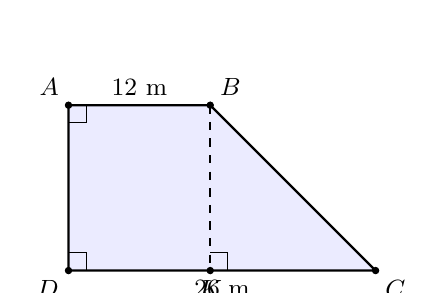
\begin{tikzpicture}[scale=0.75, font=\small]
  \coordinate (D) at (0,0);
  \coordinate (K) at (2.4,0);
  \coordinate (C) at (5.2,0);
  \coordinate (B) at (2.4,2.8);
  \coordinate (A) at (0,2.8);
  \draw[thick, fill=blue!8] (A) -- (B) -- (C) -- (D) -- cycle;
  \draw[thick, dashed] (B) -- (K);
  \draw (0,0.3) -- (0.3,0.3) -- (0.3,0);
  \draw (0,2.5) -- (0.3,2.5) -- (0.3,2.8);
  \draw (2.4,0.3) -- (2.7,0.3) -- (2.7,0);
  \filldraw (A) circle (1.5pt) node[above left] {$A$};
  \filldraw (B) circle (1.5pt) node[above right] {$B$};
  \filldraw (C) circle (1.5pt) node[below right] {$C$};
  \filldraw (D) circle (1.5pt) node[below left] {$D$};
  \filldraw (K) circle (1.5pt) node[below] {$K$};
  \node[above] at (1.2,2.8) {$12\text{ m}$};
  \node[below] at (2.6,0) {$26\text{ m}$};
\end{tikzpicture}
\end{center}
\choice
{$168\text{ m}^2$}
{$133\text{ m}^2$}
{\True $266\text{ m}^2$}
{$312\text{ m}^2$}
\loigiai{
Chiều cao $AD$ của hình thang bằng chiều rộng hình chữ nhật $ABKD$:\\$AD = 168 : 12 = 14\text{ (m)}$.\\Diện tích hình thang $ABCD$ là:\\$S = \dfrac{(12 + 26) \cdot 14}{2} = 266\text{ (m}^2\text{)}$.
}
\end{ex}

\begin{ex}
Bạn An có ngày sinh là số nguyên tố lớn nhất nhỏ hơn 20, tháng sinh của bạn là số nguyên tố nhỏ nhất. Vậy bạn An có ngày và tháng sinh là:
\choice
{Ngày 19 tháng 3}
{\True Ngày 19 tháng 2}
{Ngày 7 tháng 2}
{Ngày 7 tháng 3}
\loigiai{
Số nguyên tố lớn nhất nhỏ hơn 20 là 19, số nguyên tố nhỏ nhất là 2. Do đó An sinh ngày 19 tháng 2.
}
\end{ex}


\setcounter{ex}{0}
\vspace{2mm}
\noindent\textbf{\large PHẦN II. CÂU TRẮC NGHIỆM ĐÚNG SAI}
\vspace{1mm}
\begin{ex}
Xét tính đúng/sai của các mệnh đề sau:
\choiceTF
{\True Số $1975$ là hợp số}
{Mọi số nguyên tố đều là số lẻ}
{\True Số 1 không là hợp số cũng không là số nguyên tố}
{Tổng của hai số nguyên tố bất kì luôn là một số chẵn}
\loigiai{
\textbf{a)} Đúng. Số 1975 có chữ số tận cùng là 5 nên chia hết cho 5, ngoài ra nó còn có các ước khác 1 và chính nó như 5, 395.

\textbf{b)} Sai. Số 2 là số nguyên tố và là số chẵn.

\textbf{c)} Đúng. Theo định nghĩa, số 0 và số 1 không phải là số nguyên tố cũng không phải là hợp số.

\textbf{d)} Sai. Ví dụ $2$ và $3$ đều là số nguyên tố, nhưng tổng $2 + 3 = 5$ là số lẻ.
}
\end{ex}

\begin{ex}
Cho hình thoi $MNPQ$ có độ dài hai đường chéo lần lượt là $MP = 10\text{ cm}$ và $NQ = 6\text{ cm}$. Xét tính đúng/sai của các khẳng định sau:
\choiceTF
{\True Bốn cạnh $MN, NP, PQ, QM$ có độ dài bằng nhau}
{Hai đường chéo $MP$ và $NQ$ song song với nhau}
{\True Diện tích của hình thoi $MNPQ$ là $30\text{ cm}^2$}
{\True Hai đường chéo $MP$ và $NQ$ cắt nhau tại trung điểm của mỗi đường và vuông góc với nhau}
\loigiai{
\textbf{a)} Đúng. Hình thoi có đặc điểm là bốn cạnh đều có độ dài bằng nhau.

\textbf{b)} Sai. Hai đường chéo của hình thoi cắt nhau và vuông góc với nhau, không song song với nhau.

\textbf{c)} Đúng. Diện tích hình thoi bằng nửa tích độ dài hai đường chéo: $S = \dfrac{10 \cdot 6}{2} = 30\text{ (cm}^2\text{)}$.

\textbf{d)} Đúng. Đây là tính chất đặc trưng cơ bản về hai đường chéo của hình thoi.
}
\end{ex}


\setcounter{ex}{0}
\vspace{2mm}
\noindent\textbf{\large PHẦN III. CÂU HỎI TRẢ LỜI NGẮN}
\vspace{1mm}
\begin{ex}
Tìm số tự nhiên $x$ thỏa mãn $3 \cdot (x - 5) = 2^3 \cdot 3$. \shortans{13}
\loigiai{
Ta có: $2^3 \cdot 3 = 8 \cdot 3 = 24$.\\Biểu thức trở thành: $3 \cdot (x - 5) = 24 \Rightarrow x - 5 = 24 : 3 = 8 \Rightarrow x = 8 + 5 = 13$.
}
\end{ex}

\begin{ex}
Một hình bình hành có độ dài một cạnh bằng $10\text{ cm}$ và chiều cao tương ứng bằng $6\text{ cm}$. Tính diện tích của hình bình hành đó (theo đơn vị $\text{cm}^2$). \shortans{60}
\loigiai{
Diện tích của hình bình hành là: $S = 10 \times 6 = 60\text{ (cm}^2\text{)}$.
}
\end{ex}


\setcounter{ex}{0}
\vspace{2mm}
\noindent\textbf{\large PHẦN IV. TỰ LUẬN (BÀI TẬP VÀ BAREM ĐIỂM)}
\vspace{1mm}
\begin{ex} (0,75 điểm)
Viết tập hợp $A$ các số tự nhiên lớn hơn 9 và nhỏ hơn 15 bằng hai cách.
\loigiai{
\textbf{Cách 1 (Liệt kê các phần tử):}\\ $A = \{10; 11; 12; 13; 14\}$.\\
\textbf{Cách 2 (Chỉ ra tính chất đặc trưng):}\\ $A = \{x \in \mathbb{N} \mid 9 < x < 15\}$.
}
\end{ex}
\vspace{2mm}

\begin{ex} (1,0 điểm)
Thực hiện phép tính:
\begin{enumerate}[label=\textbf{\alph*)}, leftmargin=0.8cm, itemsep=2pt]
\item (0,5 điểm) $(30 - 10 \cdot 2) : 5$
\item (0,5 điểm) $135 \cdot 3^2 - 3^2 \cdot 130$
\end{enumerate}
\loigiai{
\textbf{a)} \textbf{[0,5 điểm]}\\ $(30 - 10 \cdot 2) : 5 = (30 - 20) : 5 = 10 : 5 = 2$.

\textbf{b)} \textbf{[0,5 điểm]}\\ $135 \cdot 3^2 - 3^2 \cdot 130 = 3^2 \cdot (135 - 130) = 9 \cdot 5 = 45$.


}
\end{ex}
\vspace{2mm}

\begin{ex} (0,75 điểm)
Một mảnh vườn hình chữ nhật có chiều dài $40\text{ m}$ và chiều rộng $30\text{ m}$.
\begin{enumerate}[label=\textbf{\alph*)}, leftmargin=0.8cm, itemsep=2pt]
\item (0,375 điểm) Tính chu vi và diện tích của mảnh vườn.
\item (0,375 điểm) Biết rằng mỗi túi hạt giống gieo vừa đủ $100\text{ m}^2$ đất và mỗi túi giá $40\,000$ đồng. Hỏi cần bao nhiêu túi hạt giống để gieo vừa hết mảnh vườn và cần bao nhiêu tiền?
\end{enumerate}
\loigiai{
\textbf{a)} \textbf{[0,375 điểm]}\\ Chu vi mảnh vườn là: $\mathcal{P} = (40 + 30) \cdot 2 = 140\text{ (m)}$.\\Diện tích mảnh vườn là: $S = 40 \cdot 30 = 1200\text{ (m}^2\text{)}$.

\textbf{b)} \textbf{[0,375 điểm]}\\ Số túi hạt giống cần dùng là: $1200 : 100 = 12\text{ (túi)}$.\\Số tiền cần mua hạt giống là: $12 \cdot 40\,000 = 480\,000\text{ (đồng)}$.


}
\end{ex}
\vspace{2mm}

\begin{ex} (0,5 điểm)
Cho các số tự nhiên: $23; 87; 64; 270; 425; 136; 2808$.
\begin{enumerate}[label=\textbf{\alph*)}, leftmargin=0.8cm, itemsep=2pt]
\item (0,125 điểm) Số nào chia hết cho 2?
\item (0,125 điểm) Số nào chia hết cho 3?
\item (0,125 điểm) Số nào chia hết cho 5?
\item (0,125 điểm) Số nào chia hết cho cả 2 và 5?
\end{enumerate}
\loigiai{
\textbf{a)} \textbf{[0,125 điểm]}\\ Các số có chữ số tận cùng là chữ số chẵn chia hết cho 2 là: $64; 270; 136; 2808$.

\textbf{b)} \textbf{[0,125 điểm]}\\ Các số có tổng chữ số chia hết cho 3 là: $87; 270; 2808$.

\textbf{c)} \textbf{[0,125 điểm]}\\ Các số có chữ số tận cùng là 0 hoặc 5 chia hết cho 5 là: $270; 425$.

\textbf{d)} \textbf{[0,125 điểm]}\\ Số có chữ số tận cùng là 0 chia hết cho cả 2 và 5 là: $270$.


}
\end{ex}
\vspace{2mm}


\begin{center}
\rule{4cm}{0.4pt}\\
\textit{--- HẾT ---}
\end{center}
\end{document}
